%%%%%%%%%%%%%%%%%%%%%%%%%%%%%%%%%%%%%%%%%
% fphw Assignment
% LaTeX Template
% Version 1.0 (27/04/2019)
%
% This template originates from:
% https://www.LaTeXTemplates.com
%
% Authors:
% Class by Felipe Portales-Oliva (f.portales.oliva@gmail.com) with template 
% content and modifications by Vel (vel@LaTeXTemplates.com)
%
% Template (this file) License:
% CC BY-NC-SA 3.0 (http://creativecommons.org/licenses/by-nc-sa/3.0/)
%
%%%%%%%%%%%%%%%%%%%%%%%%%%%%%%%%%%%%%%%%%

%----------------------------------------------------------------------------------------
%	PACKAGES AND OTHER DOCUMENT CONFIGURATIONS
%----------------------------------------------------------------------------------------

\documentclass[
	12pt, % Default font size, values between 10pt-12pt are allowed
	%letterpaper, % Uncomment for US letter paper size
	%spanish, % Uncomment for Spanish
]{fphw}

% Template-specific packages
\usepackage[utf8]{inputenc} % Required for inputting international characters
\usepackage[T1]{fontenc} % Output font encoding for international characters
\usepackage{mathpazo} % Use the Palatino font
\usepackage{setspace}

\usepackage{graphicx} % Required for including images

\usepackage{booktabs} % Required for better horizontal rules in tables

\usepackage{listings} % Required for insertion of code

\usepackage{enumerate} % To modify the enumerate environment

\usepackage{parskip}% http://ctan.org/pkg/parskip

\usepackage{amsmath}

\usepackage{caption}

\usepackage{tikz}
\newcommand*\circled[1]{\tikz[baseline=(char.base)]{
            \node[shape=circle,draw,inner sep=2pt] (char) {#1};}}

            \usepackage{enumitem}


\usepackage[ruled,portuguese,onelanguage,longend]{algorithm2e} %for psuedo code}% http://ctan.org/pkg/algorithm2e
% \makeatletter
% \renewcommand{\@algocf@capt@plain}{above}% formerly {bottom}
% \makeatother

%----------------------------------------------------------------------------------------
%	ASSIGNMENT INFORMATION
%----------------------------------------------------------------------------------------

\title{AULA 8 - Argumentação de Corretude} % Assignment title

\author{AVC, JPP, PC} % Student name

\date{} % Due date

\institute{Pontifícia Universidade Católica do Rio de Janeiro \\ Departamento de Informática} % Institute or school name

\class{Programação Modular (INF1301)} % Course or class name

\professor{Flavio Bevilacqua} % Professor or teacher in charge of the assignment

%----------------------------------------------------------------------------------------

\begin{document}

\SetEndCharOfAlgoLine{}

\maketitle % Output the assignment title, created automatically using the information in the custom commands above

%----------------------------------------------------------------------------------------
%	ASSIGNMENT CONTENT
%----------------------------------------------------------------------------------------
\begin{doublespace}


    \textbf{Objetivo:} Garantir através de uma argumentação baseada nas assertivas definidas para um código, que o bloco/programa está correto. Um programa correto gera saídas válidas para qualquer entrada. Quanto mais próximo do que o cliente quer, mais alta a qualidade do que foi feito.

    \textbf{Tipos de Argumentação:}

    \begin{itemize}

        \item Sequência
        \item Seleção
        \item Repetição

    \end{itemize}

    O descritor de estado é aquilo que indica evolução em um loop.

    \textbf{Argumentação de sequência:}

    \begin{figure}[h!]

        \centering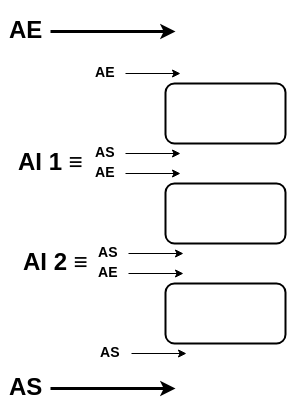
\includegraphics[scale=0.55]{argumentacaodesequencia.png}

    \end{figure}

    \begin{algorithm}[h]

        \caption{Excluir nó corrente intermediário de lista duplamente encadeada}

        \SetAlgoLined
        % \KwData{this text}
        % \KwResult{how to write algorithm with \LaTeX2e }
        AE $\longrightarrow$

        \Indp\Inicio
        {
        AJUSTA PONTEIRO NÓ ESQUERDO

        \Indm AI 1 $\longrightarrow$

        \Indp AJUSTA PONTEIRO NÓ DIREITO

        \Indm AI 2 $\longrightarrow$

        \Indp EXCLUI NÓ CORRENTE

        \Indm AI 3 $\longrightarrow$

        \Indp REDIRECIONA PONTEIRO CORRENTE

        }

        \Indm AS $\longrightarrow$

    \end{algorithm}

    AE:

    \begin{itemize}

        \item Valem as assertivas\dots
        \item Ponteiro corrente aponta para o nó a ser excluído.

    \end{itemize}

    AS:

    \begin{itemize}

        \item Valem as assertivas\dots
        \item Nó corrente foi excluído.
        \item Ponteiro corrente foi reposicionado para o primeiro nó da lista.

    \end{itemize}

    AI 1:

    \begin{itemize}

        \item Ponteiro do nó anterior ao corrente aponta para o próximo.
        \item Ponteiro para o nó anterior é nulo.

    \end{itemize}

    AI 2:

    \begin{itemize}

        \item Ponteiro do nó posterior ao corrente aponta para o anterior.
        \item Ponteiro para o nó posterior é nulo.

    \end{itemize}

    AI 3:

    \begin{itemize}

        \item Ponteiro do nó corrente é nulo.

    \end{itemize}

    \pagebreak

    \textbf{Argumentação de seleção:}

    \begin{figure}[ht]
        \begin{minipage}{0.45\linewidth}
            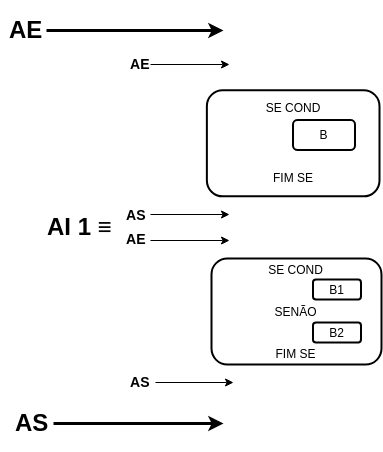
\includegraphics[width=\textwidth]{argumentacaodeselecao.png}
        \end{minipage}
        \begin{minipage}{0.5\linewidth}

            AE \&\& (Condição == True) \circled{+} B $\Longrightarrow$ AS

            AE \&\& (Condição == False) $\Longrightarrow$ AS

            \bigskip

            \bigskip

            \bigskip

            \bigskip

            \bigskip

            AE \&\& (Condição == True) \circled{+} B1 $\Longrightarrow$ AS

            AE \&\& (Condição == True) \circled{+} B2 $\Longrightarrow$ AS
        \end{minipage}
    \end{figure}

    \begin{algorithm}[h]

        \caption{Condição de ordenação}

        \SetAlgoLined
        % \KwData{this text}
        % \KwResult{how to write algorithm with \LaTeX2e }
        AE $\longrightarrow$

        \Indp\Inicio
        {
        \lSe{LISTA VAZIA}{"NÃO É POSSÍVEL ORDENAR"}
        \lSenao{ORDENA LISTA ALFABETICAMENTE}
        }
        \Indm AS $\longrightarrow$

    \end{algorithm}

    AE:

    \begin{itemize}

        \item Valem as assertivas\dots
        \item Lista pode estar vazia ou não.

    \end{itemize}

    AS:

    \begin{itemize}

        \item Valem as assertivas\dots
        \item Lista está ordenada ou mensagem foi apresentada.

    \end{itemize}

    \begin{enumerate}[label=\protect\circled{\arabic*}]
        \item AE \&\& (Condição == True) \circled{+} B1 $\Longrightarrow$ AS

              Pela AE, lista pode estar vazia. Como (Condição == True), lista está vazia. Neste caso, executa B1 que apresenta a mensagem "não é possível ordenar", valendo a AS.

        \item AE \&\& (Condição == False) \circled{+} B2 $\Longrightarrow$ AS

              Pela AE, lista pode não estar vazia. Como (Condição == False), lista possui pelo menos um elemento. Neste caso, executa B2 que ordena a lista. Vale a AS pois a lista termina ordenada.

    \end{enumerate}

    \textbf{Argumentação de repetição:}

    Tudo gira em torno do estado e do descritor de estado.

    AE: Assertiva de entrada.

    AS: Assertiva de saído.

    AINV: Assertiva invariante. Válida a cada ciclo da repetição e relacionada ao descritor de estado.

    \begin{enumerate}[label=\protect\circled{\arabic*}]
        \item AE $\Longrightarrow$ AINV
        \item AE \&\& (Condição == False) $\Longrightarrow$ AS

              (Condição == False) significa que não entrou dentro do bloco ou não concluiu o primeiro ciclo.

        \item AE \&\& (Condição == True) \circled{+} B $\Longrightarrow$ AINV

              Primeiro ciclo.

        \item AINV \&\& (Condição == True) \circled{+} B $\Longrightarrow$ AINV

              Demais ciclos

        \item AINV \&\& (Condição == False) \circled{+} B $\Longrightarrow$ AS

              Último ciclo.

        \item Término

    \end{enumerate}


\end{doublespace}
%----------------------------------------------------------------------------------------

\end{document}
